% Auth: Nicklas Vraa
% Docs: https://github.com/NicklasVraa/LiX
% Everything you need to know about this template is found in on the github repository above. Stars are very appreciated.

\documentclass{novel}

\usepackage{subfig}
\usepackage{amsmath, amsthm, amscd, amsfonts, amssymb, graphicx, color,colortbl, latexsym,multirow}
\usepackage{hyperref}
\usepackage{float}

\lang      {english}
\title     {Pactus: A Decentralized, User-Friendly, and Fair Blockchain Platform}
%\subtitle  {White Paper}
%\authors   {Pactus Research Team}
\cover     {resources/novel_front.pdf}{resources/novel_back.pdf}
\license   {CC}{by-nc-sa}{3.0}
\publisher {Pactus Blockchain}
\edition   {1}{March 2024 (Version 1.0)}
\dedicate  {all the people who try to make the world a better place to live in.}{Together we can build the decentralized Future.}
\keywords  {Pactus, Blockchain, Fairness, Consensus}

\note{Pactus is a unique and innovative project that can offer a simple, fair, and transparent solution to the challenges of centralization and complexity in the blockchain space. In Pactus, users can enjoy a user-friendly experience with the Pactus GUI application, which makes it easy to run a node and interact with the platform. For the community, Pactus fosters a decentralized and democratic governance model, where anyone can become a validator and participate in the consensus process.
Join Pactus and build the future!\\
\\Pactus Research Team}

\blurb{Pactus offers a unique and sustainable way of running a blockchain network, with faster and more scalable transactions, and smarter and more flexible contracts. Pactus is not just a technology, it’s a vision for a more secure, private, and empowered web.
}

\begin{document}

\toc
\h {Executive Summary}
Pactus is a decentralized and user-friendly blockchain platform that aims to solve the scalability, security, and complexity issues of existing blockchain networks. Pactus uses a unique consensus mechanism called Solid State Proof of Stake, which enables fast and secure block creation without the need for delegation or miners. Pactus also offers a simple GUI application that allows anyone to run a node and interact with the platform. Pactus has a percentage-based fee model that ensures fairness and predictability, and a dedicated decentralized storage feature that enables new protocols and applications in the decentralized space. Pactus has a native coin called PAC, which has a fixed supply of 42 million and is distributed through block rewards and treasury funds. Pactus is a community-run project that welcomes anyone to join and contribute to its development and growth.

\h{Introduction}

Did you know that the global blockchain market size is expected to reach 39.7 billion USD by 2025, growing at a compound annual growth rate of 67.3\% [source]. Blockchain technology has the potential to revolutionize various industries and sectors, such as finance, healthcare, supply chain, and social media. However, despite the rapid growth and innovation in the blockchain space, there are still many challenges and barriers that hinder the adoption and usability of blockchain platforms. Some of these challenges include scalability, security, complexity, centralization, and high costs.

Many existing blockchain platforms rely on slow and costly consensus algorithms that are executed on sophisticated, resource rich, high power consuming machines. This makes them less just, slow and more polluting to the environment. These mechanisms introduce the risk of centralization and manipulation, as well as consume a lot of resources and energy. Moreover, many blockchain platforms are not user-friendly and require a high level of technical knowledge and skills to use and develop. Furthermore, many blockchain platforms have a fixed or complex fee model that makes it difficult to predict and control the transaction costs.

Pactus is a blockchain platform that aims to solve these challenges and provide a decentralized and user-friendly solution for the blockchain industry. Pactus uses a unique consensus mechanism called Solid State Proof of Stake, which enables fast and secure block creation without the need for delegation or miners. Pactus also offers a simple GUI application that allows anyone to run a node and interact with the platform. Pactus has a percentage-based fee model that ensures fairness and predictability, and a dedicated decentralized storage feature that enables new protocols and applications in the decentralized space. Pactus has a native coin called PAC, which has a fixed supply of 42 million and is distributed through block rewards and treasury funds. Pactus is a community-run project that welcomes anyone to join and contribute to its development and growth.

The purpose of this white paper is to provide a detailed and comprehensive explanation of the Pactus project and its technology. This white paper is intended for anyone who is interested in learning more about Pactus and its potential, such as investors, developers, users, and enthusiasts. By reading this white paper, you will gain a better understanding of the problem that Pactus is solving, the solution that Pactus is offering, and the benefits that Pactus is bringing to the blockchain industry and the society.

This white paper is divided into the following sections:
\begin{itemize}
  \item
        Pactus: This section explains the problem that Pactus is solving and how Pactus works as a solution. It also compares Pactus with some of the existing blockchain platforms and highlights the advantages and disadvantages of each platform.
  \item
        Consensus Algorithm: This section describes the technical aspects of Pactus, such as the architecture, the protocol, the consensus mechanism, the security, and the scalability. It also provides some examples and diagrams to illustrate how Pactus works and operates.
  \item
        Roadmap: This section outlines the milestones and the timeline of the project development. It also mentions any challenges or risks that the project anticipates and how the project plans to overcome them.
  \item
        Tokenomics: This section explains the token model of Pactus, such as the type, the supply, the distribution, the value, and the use cases. It also explains how Pactus aligns the incentives of the network and supports the growth of the project.
  \item
        Conclusion: This section summarizes the white paper and the unique values proposed by the Pactus.
\end{itemize}

We hope that this white paper can provide you with a clear and comprehensive understanding of the Pactus project and its potential. We welcome any feedback, questions, or suggestions that you may have. To contact and join us visit pactus.org.

\h{Pactus: The future of the Decentralization}
In this section, we will provide some background information on Pactus, its mission, vision, and values. We will also explain why is it recommended to join Pactus.

\subsection{What is Pactus?}
Decentralization is one of the core values and principles of blockchain technology. It refers to the distribution of power and control among the participants of a network, rather than a single authority or entity. Decentralization enables trustless, transparent, and democratic systems that can resist censorship, corruption, and manipulation.

However, not all blockchain platforms are truly decentralized. Many of them rely on mechanisms that introduce the possibility of centralization and compromise the security and performance of the network. For example, some platforms use delegation or mining to achieve consensus, which can create a concentration of power and influence among a few nodes or entities. Moreover, some platforms have a complex or fixed fee model, which can create a barrier for entry and participation for many users.

Pactus is a blockchain platform that aims to achieve the highest level of decentralization possible, while maintaining a high-performance, secure, and user-friendly system. Pactus has several unique characteristics that make it stand out from other blockchain platforms:

\begin{itemize}
\item Pactus uses a novel consensus mechanism called Solid State Proof of Stake (SSPoS), which enables fast and secure block creation without the need for delegation or miners. SSPoS is based on the concept of solid state, which means that the state of the network is determined by the validators and their stakes, rather than by the blocks or the transactions. This allows the network to reach consensus in a matter of seconds, without wasting resources or energy. SSPoS also ensures that anyone can become a validator and participate in the consensus process, as long as they have a minimum stake of 1 PAC coin. This creates a fair and inclusive system that prevents centralization and manipulation.
\item Pactus offers a simple GUI application that allows anyone to run a node and interact with the platform. The Pactus GUI application is designed to be easy to use and maintain, and does not require any technical knowledge or skills. The application enables users to create and manage their wallets, send and receive transactions, run smart contracts, and monitor the network status. The application also allows users to become validators and join the consensus process with a few clicks. The Pactus GUI application makes Pactus accessible and convenient for anyone, regardless of their background or experience.
\item Pactus has a percentage-based fee model that ensures fairness and predictability. Transaction fees are calculated based on a percentage model with a minimum and maximum fee. These parameters provide greater control over the fee structure and prevent overpaying or underpaying. The percentage-based model ensures that the fees are proportional to the value of the transactions, and that the fees are distributed among the validators and the treasury fund. The percentage-based model can also be adjusted through consensus among all validators, ensuring that the platform remains responsive and adaptive to the market conditions and the user preferences.
\item Pactus has a dedicated decentralized storage feature that enables new protocols and applications in the decentralized space. In Pactus, users can purchase a dedicated storage file that can be renewed annually, leading to reduced costs for storage and smart contract execution. This unique feature can pave the way for new protocols and applications that require large amounts of data or computation, such as decentralized social media, decentralized cloud computing, or decentralized artificial intelligence.
\end{itemize}

\subsection{Mission and Vision}
The mission of Pactus is to create a decentralized and user-friendly blockchain platform that can empower anyone to participate in the ecosystem and benefit from the technology. The vision of Pactus is to become the future of decentralization, where anyone can create, share, and exchange value and data in a simple, fair, and transparent way.

\subsection{Why join Pactus?}
We recommend anyone who is interested in blockchain technology and decentralization to join and use Pactus. By joining Pactus, you will become a part of a vibrant and diverse community that values innovation, collaboration, and inclusion. You will also be able to access and enjoy the features and benefits of Pactus, such as fast and secure transactions, low and predictable fees, dedicated decentralized storage, and user-friendly GUI application. You will also have the opportunity to contribute to the development and growth of Pactus, by becoming a validator, a developer, or a supporter. Pactus is more than just a blockchain platform, it is a movement and a vision for the future of decentralization.

\h{Consensus Algorithm: Solid State Proof of Stake (SSPoS)}
In this section, we introduce the consensus algorithm of the Pactus, called Solid State Proof of Stake (SSPoS).
\subsection{Overview}
A consensus algorithm is a mechanism that allows a distributed network of nodes to agree on the state and the validity of the transactions and the blocks. A consensus algorithm is essential for ensuring the security, performance, and decentralization of a blockchain platform.

There are different types of consensus algorithms, such as Proof of Work, Proof of Stake, Delegated Proof of Stake, and others. Each of them has its own advantages and disadvantages, such as speed, energy consumption, scalability, and centralization.

\textbf{Proof of Stake:} To understand how Proof of Stake works, imagine a community bank without any centralized authority. In this bank, users decide to run it together. Some of these users volunteer to collect, validate, and record transactions, ensuring that everything runs smoothly.

These volunteers, known as validators, must temporarily lock or freeze some of their money as a stake. This stake can’t be transferred or used. The more money a validator stakes, the more influence they have in the system.

From time to time, one of the validators is chosen by the others to collect all the recent transactions, bundle them together, and send a copy to the other validators. If a supermajority of the validators agree with the proposed bundle by signing it, the bundle will be committed to the bank’s ledger. In this system, validators have no incentive to behave maliciously or dishonestly. If they do, they risk harming the bank’s reputation and the value of their own stakes as well.

\textbf{Delegated Proof of Stake:} In Proof of Stake, if the number of validators increases, the voting time will also increase, and this can lead to an inefficient consensus mechanism. In our community bank example, running the bank becomes more difficult as the number of validators increases.
\begin{figure*}[h]
	\centering
	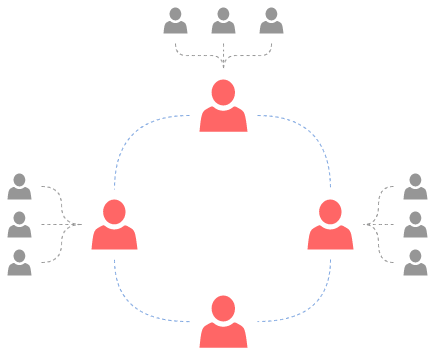
\includegraphics[scale=0.5]{dpos.png}
	\caption{Overflow of Delegated Proof of Stake }
	\label{fig:dpos}
	\centering
\end{figure*}

To solve this problem, some blockchains use the concept of “delegators”. In Delegated Proof of Stake, users entrust their stakes to a small group of “delegates”. Figure~\ref{fig:dpos} shows the overview of Delegated Proof of Stake. These delegates are responsible for validating transactions and creating blocks. The number of delegates is limited to ensure accountability and efficiency in the validation process.

The delegation model puts a lot of trust in the hands of a small number of delegates, which goes against the principle of “don’t trust, verify”.
	
\textbf{Pactus Algorithm:} Pactus introduced a mechanism that doesn’t rely on delegation, we call it Solid State Proof of Stake. The SSPoS is a state machine replication with Byzantine fault tolerance, shown in Figure~\ref{fig:pcs}. The Pactus consensus algorithm starts with the block creation phase. In this phase one validator acts as the proposer. The proposer collects all the transactions, creates a block, and proposes it to other validators.

%
%\begin{figure*}[h]
%	\centering
%	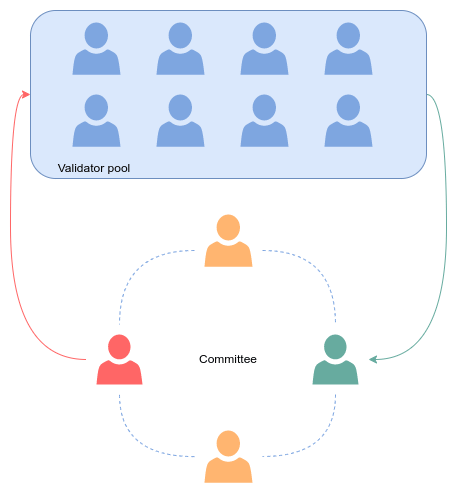
\includegraphics[scale=0.5]{pvp.png}
%	\caption{Pactus validators pool }
%	\label{fig:pvp}
%	\centering
%\end{figure*}
\begin{figure*}[h]
	\centering
	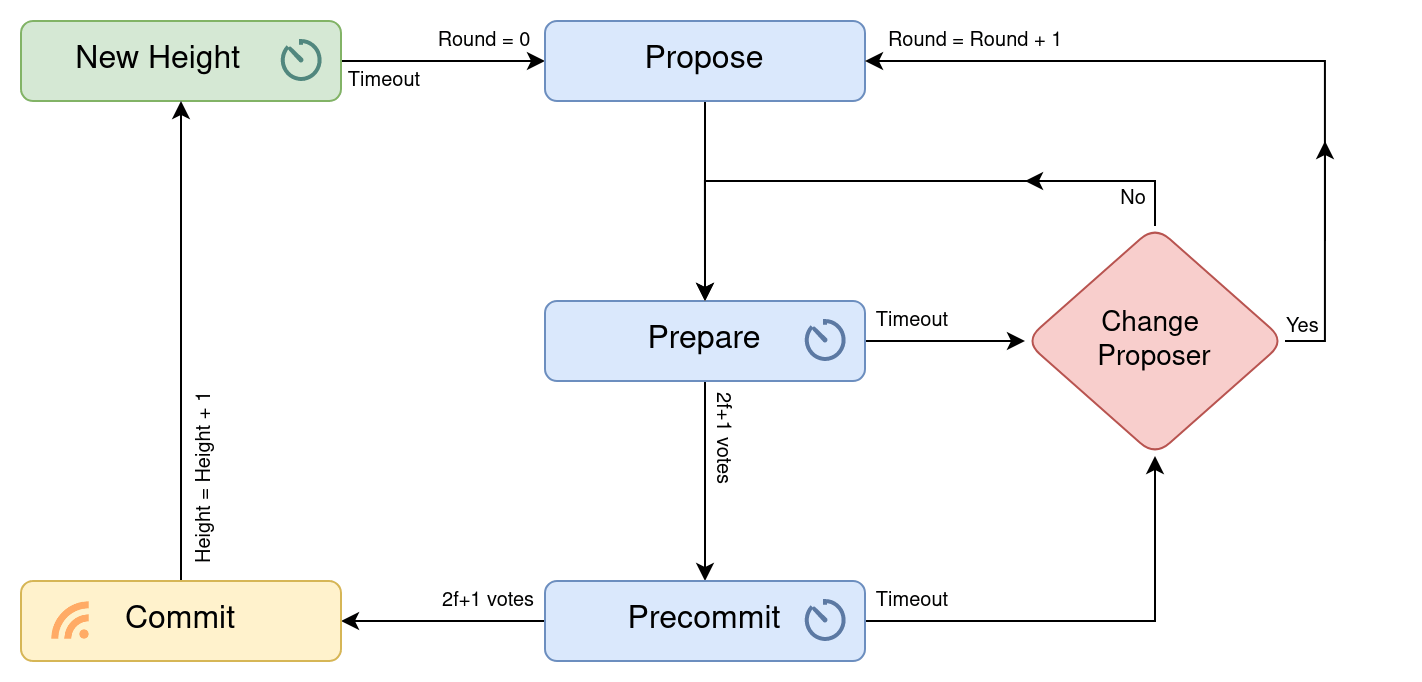
\includegraphics[scale=0.23]{pcs.png}
	\caption{Pactus Consensus States }
	\label{fig:pcs}
	\centering
\end{figure*}

When a proposed block is seen by other validators, they validate the block and cast their vote for the proposed block, moving to the “prepare” state.

If more than two-thirds ($\frac{2}{3}$) of the total stakes cast their votes, the proposed block becomes prepared, and validators move to the “precommit” state.

If, once again, more than two-thirds($\frac{2}{3}$) of the total stakes cast their vote for the prepared block, the block is committed, and the next proposer is ready to propose a new block. This cycle repeats every 10 seconds.

If a proposer fails to propose in any round, other validators start the “change proposer” phase to decide to change the proposer for this round.

\subsection{Solid State Proof of Stake algorithm}
There are $R = 3f+1$  validators. where $f$ is the maximum number of validators that may be faulty or byzantine. For example, if there is one faulty validator, the resiliency of the algorithm is optimal if we have at least 3 non-faulty validators. So the minimum number of validators should be $3+1=4$.

We denote a message as $\langle m \rangle$ tuple and a signed message by node $i$ as $\langle m \rangle_{\sigma_i}$.

Pactus consensus algorithms has two phases: Block creation phase and change proposer phase.

\subsubsection{Block Creation}
The block creation phase in Pactus consensus algorithm includes these three steps1: \emph{Propose}, \emph{Prepare} and \emph{Precommit}. The protocol proceeds in rounds $r = 0, 1, 2, \ldots$.


\noindent \emph{Propose Step:} f validator $i$ accepts the proposal, it enters the prepare step and signs and broadcasts the prepare message to all other validators. Otherwise, it does nothing. The prepare message has this form:
\begin{equation*}
  \langle \text{PREPARE},h,r,d \rangle_{\sigma_i}
\end{equation*}
where
\begin{itemize}
  \item $B$ is the proposed block.
  \item $h$ indicates the block height.
  \item $r$ is an assigned round number, which is zero for the first round.
\end{itemize}

\noindent \emph{Prepare Step:} If validator $i$ accepts the proposal, it enters the prepare step and signs and broadcasts the prepare message to all other validators. Otherwise, it does nothing. The prepare message has this form:
\begin{equation}
  \langle \text{PREPARE},h,r,d \rangle_{\sigma_i}
\end{equation}
where
\begin{itemize}
  \item $d$  is the digest or hash of the proposed block $B$.
\end{itemize}
If validator $i$ received $2f+1$ prepare messages from other validators (including its own), it becomes \emph{prepared} and enters to precommit step.

\noindent \emph{Precommit Step:}In precommit step, validator $i$ signs and broadcasts precommit message to the other validators. The precommit message has this form:
\begin{equation*}
  \langle \text{PRECOMMIT},h,r,d \rangle_{\sigma_i}
\end{equation*}
Each validator executes and commits block $b$ after receiving $2f+1$ precommit messages (including its own) and becomes \emph{committed}.

\noindent \emph{Block Announcement:} Each validator that receives a valid proposal and with $2f+1$ precommit messages from other validators (including its own), can create a block-announce messages and broadcasts it to the network. The block-announce message has this form:
\begin{equation*}
  \langle \text{BLOCK-ANNOUNCE} ,h ,r ,B, C \rangle
\end{equation*}
where
\begin{itemize}
  \item $C$ is the quorum certificate for the precommit step.
\end{itemize}
Validators can move to the next height and clear the message logs after receiving A valid block-announce message, even if their timer has expired.

\begin{figure*}[!t]
	\centering
	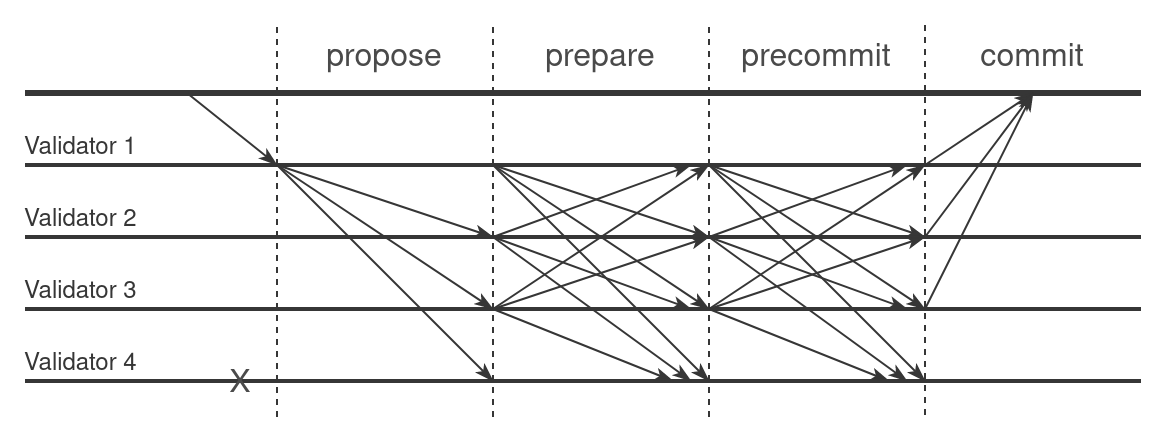
\includegraphics[scale=0.3]{normop.png}
	\caption{SSPoS Normal Execution}
	\label{fig:normop}
	\centering
\end{figure*}


Figure~\ref{fig:normop} below shows the operation of the algorithm in the normal case. validator 1 is the proposer and validator 4 is faulty.

\subsubsection{Change-Proposer}
The change-proposer provides liveness by allowing the system to make progress when the proposer fails. The change-proposer phase is triggered by timeouts that prevent validators from waiting indefinitely for the proposal to execute.

If the timer of a validator expires in round $r$, the validator starts a change-proposer phase. The change-proposer phase is an Asynchronous Byzantine Binary Agreement (ABBA) that is biased toward zero (No). It means that during this phase, even if they don’t have the proposal, honest validators may decide to vote zero if they obtain a valid quorum Certificate for the prepare step.

If a supermajority of the validators decide to change the proposer, they move to round $r+1$. However, if they decide not to change the proposer, they will return to the prepare state and, since a supermajority of the validators attested to a valid proposal, they can commit the proposed block.

The change proposer phase in Pactus consensus algorithm includes these three steps: \emph{Pre-vote}, \emph{Main-vote}, and \emph{Decide}. The protocol proceeds in rounds $r_{cp} = 0, 1, 2, \ldots$.

\noindent \emph{Pre-vote Step:} In Pre-vote step each validator casts a pre-vote for a value $b \in \{0, 1\}$ and broadcasts a pre-vote message to the network. The pre-vote message has this form:
\begin{equation*}
  \langle\langle \text{CP:PRE-VOTE},h,r,r_{cp},b \rangle_{\sigma_i}, justification\rangle
\end{equation*}

The first round is a special round and each validator starts with an initial value. If the validator’s timer has expired in the prepare step, its initial value is zero, and if the validator’s timer has expired in the precommit step, its initial value is one.

\begin{equation}
  b = \begin{cases}
        1 & \text{if timer expired in prepare step,} \\
        0 & \text{if timer expired in precommit step.}
      \end{cases}
\end{equation}

In the next rounds, each validator selects $2f+1$ properly justified main-votes from the round $r-1$ and
\begin{equation*}
  b = \begin{cases}
        0 & \text{if there is a main-vote for 0,} \\
        1 & \text{if there is a main-vote for 1,} \\
        0 (biased) & \text{if all main-votes are abstain.}
    \end{cases}
\end{equation*}

These pre-votes must be justified with an appropriate justification. For the first round, if the validator’s timer has expired in the prepare step, the justification is $nil$, and if the validator’s timer expired in the precommit step, the justification is the proper quorum certificate for the prepare step at round $r$.

In the next rounds, a pre-vote for $b$ may be justified in two ways:
\begin{itemize}
  \item \textbf{Hard}: that is the quorum certificate for $\langle \text{CP:PRE-VOTE},h,r,r_{cp}-1,b \rangle$
  \item \textbf{Soft}: that is the quorum certificate for $\langle \text{CP:MAIN-VOTE},h,r,r_{cp}-1,abstain \rangle$
\end{itemize}

\noindent \emph{Main-vote Step:} After collecting $2f+1$ valid and justified pre-votes, each validator casts a main-vote $v \in \{0, 1, abstain\}$ and broadcasts main-vote message to the network. The main-vote message has this form:
\begin{equation*}
  \langle\langle \text{CP:MAIN-VOTE},h,r,r_{cp},v \rangle_{\sigma_i}, justification\rangle
\end{equation*}
The main-vote value $v$ is determined as below:
\begin{equation*}
  v = \begin{cases}
    0 & \text{if there are 2f+1 pre-vote for 0,} \\
    1 & \text{if there are 2f+1 pre-vote for 1,} \\
    abstain & \text{if there are pre-votes for 0 and 1.}
    \end{cases}
\end{equation*}
These main-votes must be justified with a appropriate justification. A main-vote for $v$ may be justified in two ways:
\begin{itemize}
  \item \textbf{Non-conflicting:} that is the quorum certificate for $\langle \text{CP:PRE-VOTE},h,r,r_{cp},b \rangle$
  \item \textbf{Conflicting}: that consists of the justifications for the two conflicting pre-votes.
\end{itemize}
\noindent \emph{Decide Step:} After collecting $2f+1$ valid and justified main-votes, each validator examines these votes. If all votes are for a value $b \in \{0, 1\}$, then the validator decides $b$, but continues to participate in the protocol for one more round. Otherwise, the validator proceeds to the next round $r_{cp}+1$.

\subsubsection{Comparison}
Pactus consensus protocol doesn’t have any locking mechanism or checkpointing and there will be at most one valid proposal per round. This ensures that each round can begin with a new proposal.

\begin{tabular}{|p{1.8cm}|p{1cm}|p{2.5cm}|p{2cm}|p{3cm}|  }
 \hline
 & \multicolumn{2}{c|}{\textbf{Normal Case}}&\multicolumn{2}{|c|}{\textbf{Faulty case}}\\
 \hline
 \textbf{Protocol} & \textbf{Steps} & \textbf{Complexity} & \textbf{Locking} & \textbf{Checkpointing} \\
 \hline
 PBFT & 3 & $O(n^2)$ & No & Yes \\
 \hline
 Tendermint & 3 & $O(n^2)$ & Yes & No \\
 \hline
 HotStuff & 4 & $O(n)$ & Yes & No \\
 \hline
 \textbf{Pactus} & 3 & $O(n^2)$ & No & No \\
 \hline
\end{tabular}

\subsection{Specification}
Developing distributed and concurrent systems is a complex task that requires careful attention to the details. Testing such systems is challenging because it’s difficult to simulate all possible states, including those that can happen due to system failures, network latency, and other factors. This makes it hard to ensure that the system behaves correctly in all circumstances.

Therefore it’s essential to have a proactive approach that involves modeling the system’s behavior in a formal way. Such an approach can help identify potential issues before they occur, saving time and preventing costly flaws.

TLA+ is a formal specification language developed by Leslie Lamport based on the idea of specifying systems using simple mathematics. It is used for designing, modelling, documentation, and verification of programs, especially concurrent and distributed systems. TLA+ and its tools are useful for eliminating fundamental design errors, which are hard to find and expensive to correct in code.

Pactus consensus specification has been written in TLA+ format. It includes all invariants that can be held in every state of every execution that the protocol allows. The TLA+ specification is compiled into a PDF file and is available on pactus.org.

\noindent \textbf{Safety Proof:} By defining some invariants we can ensure the safety of the consensus protocol in any possible and distinct state, and therefore we have the informal safety proof of the Pactus consensus protocol using TLA+.

\noindent \textbf{Liveness Proof:} Checking the liveness is not easy, but with defining some constraints, we have the informal proof of liveness of Pactus consensus protocol using TLA+.

\subsection{Sortition Algorithm}
The sortition algorithm is an important part of the Pactus blockchain, responsible for the fair, transparent and random selection of validators to join the committee. It utilizes a Verifiable Random Function, or VRF for short, to generate a verifiable random number.

The generated random number should be in the range of 0 to the total staked coins. If validators can prove that their generated number is less than their stake, they can send the sortition transaction. Once a sortition transaction is included in a block, the validator will join the committee, and the oldest validator in the committee will leave it.

\subsubsection{Verifiable Random Function}
Verifiable Random Function is a pseudo-random function that the owner of key $s$ can evaluate $v = f_s(x)$ and also provides $proof_{x}$  efficiently proving that $v$ is correct. We call such a mathematical object a verifiable pseudo-random function, VRF for brevity.

Pactus uses the BLS signature scheme as the source of VRF. Since BLS signatures are unique, the hash of a BLS signature can be used to produce a secure and verifiable random number.

The VRF takes three parameters:
\begin{enumerate}
  \item The secret key of the validator
  \item The sortition seed
  \item The total stake of the blockchain.
\end{enumerate}
Once the VRF is executed, it produces an index with a proof. The index is a number between zero and the total staked coins, and the proof allows other validators to verify the correctness of the generated index.

The pseudocode below demonstrates the evaluation of the VRF for the sortition algorithm:
\begin{align*}
& \textbf{function} \ VRF(sk, seed, total\_stake) \\
& \qquad pk \gets P_{BLS}(sk) \\
& \qquad proof \gets S_{BLS}(sk, seed \| pk) \\
& \qquad rnd \gets H(proof) \\
& \qquad index \gets \frac{(rnd \times total\_stake)}{2^{256}} \\
& \qquad \\
& \qquad \textbf{return} \ index, proof \\
& \textbf{end function}
\end{align*}
where
\begin{itemize}
  \item $sk$ is the secret key of the validator.
  \item $seed$ is the sortition seed.
  \item $total\_stake$ is the total stake of the blockchain.
  \item $P_{BLS}$ is a cryptographic function that derives the public key from the secret key for the BLS signature.
  \item $S_{BLS}$  is a cryptographic function that signs a message with the secret key for the BLS signature.
  \item $H$ is a cryptographic hash function that generates a number between $0$ and $2 ^{256}$.
  \item $||$ denotes the concatenation of two values.
\end{itemize}
To verify a sortition proof, both the validator’s public key and stake are required:

  \begin{align*}
    & \textbf{function} \ verifyVRF(pk, seed, proof, stake, total\_stake) \\
    & \qquad \textbf{if} \ V_{BLS}(pk, seed \| pk, proof) = True \ \textbf{then} \\
    & \qquad \qquad rnd \gets H(proof) \\
    & \qquad \qquad index \gets \frac{(rnd \times total\_stake)}{2^{256}} \\
    & \qquad \\
    & \qquad  \qquad \textbf{return} \ index \leqslant stake \\
    & \qquad  \textbf{else} \\
    & \qquad  \qquad \textbf{return} \ False \\
    & \qquad  \textbf{end if} \\
    & \textbf{end function}
\end{align*}

where
\begin{itemize}
  \item  $V_{BLS}$ is a cryptographic function used to verify a signed message using the BLS signature scheme.
\end{itemize}
There is no need to send $index$ alongside $proof$, because the result should be less than the validator’s stake, and the validator’s stake is known at each block.

\subsubsection{Sortition Seed}
The sortition algorithm relies on a random and publicly verifiable seed that cannot be manipulated by adversaries. Otherwise, adversaries may select a seed that favors the selection of corrupt users.

To prevent this, the BLS signature scheme is used to generate the sortition seed. Since BLS signatures are unique and deterministic, adversaries cannot generate more than one valid signature per block. In each block, the block proposer generates a new sortition seed based on the previous seed using the following function:

  \begin{align*}
& \textbf{function} \ generateSeed(sk, prev\_seed) \\
& \qquad \textbf{return} \ S_{BLS}(sk, H(prev\_seed)) \\
& \textbf{end function}
\end{align*}

Since the proposer’s public key is known, the seed for the next block can be easily verified. If the seed is invalid, the proposed block will be rejected. The verification function is as follows:
  \begin{align*}
& \textbf{function} \ verifySeed(pk, prev\_seed, seed) \\
& \qquad \textbf{return} \ V_{BLS}(pk, H(prev\_seed), seed) \\
& \textbf{end function}
\end{align*}

The sortition seed for the genesis block is set to $0$.

\subsubsection{Sortition Probability}
The Sortition probability refers to the expected number of validators that may join the committee in each block, assuming all validators are actively online and executing the sortition algorithm.

The probability of a validator $i$ being selected depends on their stake relative to the total stake in the system:
\begin{equation*}
  p_i=\frac{S_i}{S_t}
\end{equation*}

where:
\begin{itemize}
  \item $p_i$ is the probability of validator $i$ being selected,
  \item $S_i$ is the stake of validator $i$,
  \item $S_t$ is the total stake of all validators.
\end{itemize}

Therefore, the expected number of validators joining the committee at each block can be represented as:
\begin{equation*}
  P=\sum_{i=1}^{n}{p_i}=\sum_{i=1}^{n}{\frac{S_i}{S_t}}=\frac{S_1+S_2+\ldots+S_n}{S_t}
\end{equation*}
where $n$ is the total number of validators. We know that $S_t={S_1+S_2+\ldots+S_n}$. Therefore we will have:
\begin{equation*}
  P=\frac{S_t}{S_t}=1
\end{equation*}

Thus, on average, we expect one validator to join the committee at each block. In practice, the actual number of validators joining the committee in each block may differ due to the randomness in the sortition algorithm, or the possibility of some validators being offline.

\subsubsection{FAQ}
\noindent \textbf{How is the total staked coin calculated?}\\
The total staked coin in each block is calculated by summing the staked coins of all active validators. An active validator is a validator that has not yet been unbonded.

\noindent \textbf{How is the oldest validator determined?}\\
The height at which the validator joined the committee is recorded as the “Last Joined Height” field in the validator structure. The validator with the lowest “Last Joined Height” is considered the oldest.



\subsection{Committee}
The committee is a group of 51 validators responsible for generating new blocks. Validators in the committee participate in the consensus algorithm by casting votes, with their voting power determined by their stake. While in the committee, validators cannot send Bond or Unbond transactions, meaning their voting power remains the same. The members of the committee change randomly over time through Sortition transactions. Each block can contain zero or more Sortition transactions.

These rules are applied when committing sortition transactions:
\begin{enumerate}
  \item A minimum of $\frac{2}{3}$ of the total stake must be maintained in the committee.
  \item If a validator is already in the committee, they will remain in the committee.
  \item If a validator is not in the committee, the oldest validator will exit the committee.
  \item Each validator should stay in committee at least for 51 blocks.
\end{enumerate}
\begin{figure*}[h]
	\centering
	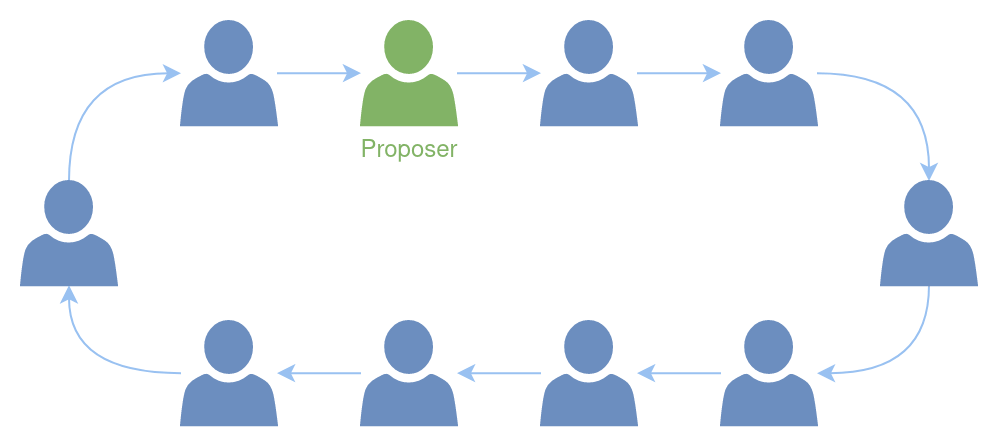
\includegraphics[scale=0.25]{ps.png}
	\caption{Proposer Selection Process}
	\label{fig:ps}
	\centering
\end{figure*}

\subsubsection{Proposer Selection}
Proposer selection within the committee operates on a deterministic, clockwise rotation system. If a validator is unable to propose, for any reason, it stays within the committee, but the proposer’s role shifts to the next validator in the committee. Figure~\ref{fig:ps} shows the process of proposer selection.

\begin{figure*}[h]
	\centering
	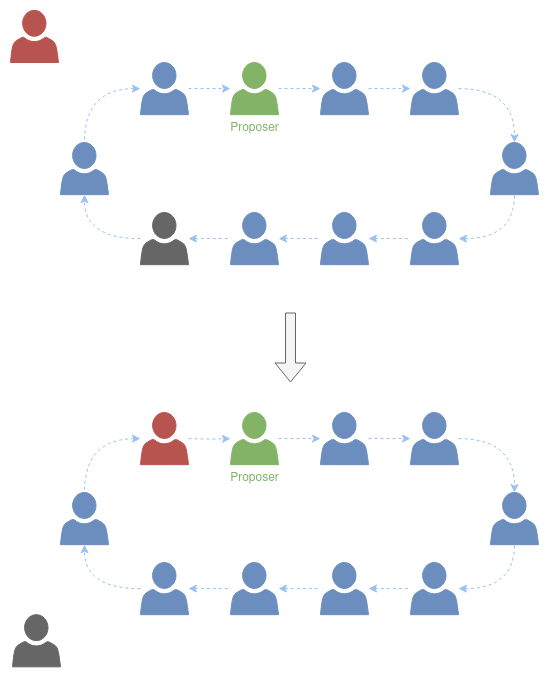
\includegraphics[scale=0.4]{cav.png}
	\caption{Adding Validators to the Committee}
	\label{fig:cav}
	\centering
\end{figure*}

\subsubsection{Adding Validators to the Committee}
When a new validator joins the committee, they take a position before the current proposer. After the addition of a new validator, the committee adjusts to maintain the total number of validators at 51. This is achieved by removing the oldest validator from the committee, i.e., the one that has been in the committee for the longest time. Figure~\ref{fig:cav} shows how a validator is added to the Committee.

\subsubsection{Security of the Committee}
For an adversary to take control of the committee, they would need to control more than $\frac{2}{3}$ of the stake within the committee. To assess the security of the committee, let’s assume all validators in the committee have the same voting power. In this case, an adversary would need to control more than $\frac{2}{3}$ of the validators in the committee.

Now, let’s imagine an adversary holds 10\% of the total stake. As a result, one of their validators can enter the committee every 10 blocks. In the first 10 blocks, one of the adversary’s validators enters the committee. In the next 10 blocks, another validator enters the committee, giving the adversary two validators within the committee. In the subsequent 10 blocks, another validator enters, but at the same time, the first validator leaves the committee. Therefore, an adversary with 10\% of the total stake can have, on average, two validators in a committee of 51 validators.

Using the Poisson distribution, we can estimate the probability of an adversary controlling $\frac{2}{3}$ of the committee:

\begin{tabular}{|p{2.1cm}|p{1.7cm}|p{2.5cm}|p{2cm}|p{2.5cm}|  }
 \hline
 \textbf{Adversarial Stake} & \textbf{Committee size} & \textbf{$\frac{2}{3}$ + of committee} & \textbf{Adversarial committee members} & \textbf{Probability of controlling $\frac{2}{3}$+} \\
 \hline
 15\% & 21 & 15 & 3 & $5.46 \times 10^{-07}$ \\
 \hline
 15\% & 51 & 35 & 7 & $3.34 \times 10^{-14}$ \\
 \hline
 15\% & 99 & 67 & 14 & $1.41 \times 10^{-24}$ \\
 \hline
 10\% & 21 & 15 & 2 & $3.39 \times 10^{-09}$ \\
 \hline
 10\% & 51 & 35 & 5 & $1.90 \times 10^{-18}$ \\
 \hline
 10\% & 99 & 67 & 9 & $2.91 \times 10^{-35}$ \\
 \hline
 5\% & 21 & 15 & 1 & $2.81 \times 10^{-13}$ \\
 \hline
 5\% & 51 & 35 & 2 & $4.50 \times 10^{-31}$ \\
 \hline
 5\% & 99 & 67 & 4 & $1.09 \times 10^{-56}$ \\
 \hline
\end{tabular}

\subsubsection{FAQ}
\noindent \textbf{How can one know when a validator has joined the committee?}\\
The height at which the validator joined the committee is recorded as the “Last Joined Height” field in the validator structure. Once a validator enters the committee, this field is set to the current height it evaluated the sortition proof.

\noindent \textbf{Can a validator within the committee run the sortition algorithm?}\\
A validator within the committee can run the sortition algorithm. If they generate a valid sortition transaction, the height of their entry into the committee is set to the current block height, allowing them to stay in the committee for a longer period.

\subsection{Consensus Parameters}
Consensus parameters are a set of configurable settings that determine how the Pactus blockchain operates. These parameters are agreed upon by all validators in the network, ensuring that validators behave in the same way and that the network operates consistently.

Here is the list of the consensus parameters:
\begin{itemize}
  \item
    \textbf{Block Version:} The version number of the blockchain protocol. This is set to 1.
  \item
    \textbf{Block Time:} The time interval in seconds between the creation of two consecutive blocks. This is set to 10 seconds, which means that a new block is created every 10 seconds.
  \item
    \textbf{Committee Size:} The number of validators in the committee. This is set to 51 validators.
  \item
    \textbf{Block Reward:} The fixed reward amount given to the validator who successfully creates and proposes a new block. This is set to 1,000,000,000, which is equivalent to one coin.
  \item
    \textbf{Time-to-Live Interval:} The number of blocks that a transaction can remain unprocessed before it is removed from the transaction pool. This is set to 8640 blocks, which is almost one day.
  \item
    \textbf{Bond Interval:} The minimum number of blocks that must elapse after a validator has submitted a bond transaction before they can participate in the consensus process and join the validator committee. This is set to 360 blocks, which is almost one hour.
    \textbf{Unbond Interval:} The minimum number of blocks that must elapse after a validator has submitted an unbond transaction before they can withdraw their staked coins. This is set to 181440 blocks, which is almost 21 days.
  \item
    \textbf{Sortition Interval:} The maximum number of blocks that a sortition transaction can remain valid and be included in a block. This is set to 7 blocks.
  \item
    \textbf{Fee Fraction:} The fraction of transaction value that must be paid in order for a transaction to be included in a block. This is set to 0.0001 PAC, meaning that 0.01\% of transaction value are awarded to the block proposer.
  \item
    \textbf{Minimum Fee:} The minimum transaction fee that must be paid. This is set to 1,000 (satoshi), which is equivalent to 0.000001 PAC coin.
  \item
    \textbf{Maximum Fee:} The maximum transaction fee that must be paid. This is set to 1,000,000 (satoshi), which is equivalent to 0.001 PAC coin.
  \item
    \textbf{Maximum Stake:} The maximum amount of coins that can be staked by a validator. This is set to 1,000,000,000,000 (satoshi), which is 1000 PAC coins.
  \item
    \textbf{Minimum Stake:} The minimum amount of coins that can be staked by a validator. This is set to 1,000,000,000 (satoshi), which is 1 PAC coins.
\end{itemize}


\h{Roadmap of Pactus}

Pactus is a blockchain platform that is constantly evolving and improving. We have a clear and ambitious roadmap that outlines the milestones and the timeline of our project development. Our roadmap is divided into four phases: Alpha, Beta, Gamma, and Delta. Each phase represents a major update or upgrade of our platform, with new features, enhancements, and optimizations.

\subsection{Alpha Phase: 2020 to 2022 (The Birth of an Idea)}
The Pactus project started in 2020 with the goal of creating a real Proof-of-Stake blockchain that anyone can be a part of in the ecosystem. Since Pactus had a unique consensus mechanism, the project couldn’t be copied or forked from existing blockchain projects. Therefore, the entire codebase and infrastructure had to be built from scratch. In the first phase, the development team focused on building a robust and stable infrastructure aimed at being easy to develop and test. This phase ended with the launch of the first testnet, which we called testnet-0\footnote{https://pactus.org/2022/09/24/testnet-0-launched.html}. The main goals of the alpha phase were:
\begin{itemize}
  \item
        Implementing the infrastructure of the Pactus blockchain by focusing on the simplicity of the codebase and ease of understanding for developers.
  \item
        Focusing on testing the project and ensuring that all possible scenarios could be tested during implementation.
  \item
        Reducing the cost of maintaining the project and the entire infrastructure.
  \item
        Designing and implementing the Solid State Proof-of-Stake consensus protocol.
  \item
        Launching the first Testnet.
\end{itemize}

\subsection{Beta Phase: 2022 to 2024 (The Establishment)}
The Beta phase is the second phase of our project development, which started in 2022 and ended in 2024. The Beta phase focuses on preparing Pactus for the Mainnet launch. The Beta phase involved the launch of Testnet-1\footnote{https://pactus.org/2023/05/09/testnet-1-launched.htm} and Testnet-2\footnote{https://pactus.org/2023/10/15/testnet-2-launched.html}, which paved the way for launching the mainnet and the official release of the platform to the public. The main goals of the Beta phase are:
\begin{itemize}
  \item
        Ensuring the stability, safety, and efficiency of the consensus mechanism in real situations with over 1000 validators.
  \item
        Ensuring peer-to-peer networking performance in real situations and reducing the networking bandwidth to make Pactus usable with a home connection.
  \item
        Assessing the security and performance of the committee and evaluating the rotation of committee members based on their stake.
  \item
        Determining the actual block creation time.
  \item
        Ensuring a smooth syncing process for new nodes joining the network.
  \item
        Evaluating transaction performance and maximum transactions per block.
  \item
        Designing a graphical user interface for beginner users to be able to run Pactus.
  \item
        Preparing for the launch of the Pactus mainnet, which will allow anyone to use and benefit from our platform and its features.
\end{itemize}

The Beta phase is the second phase of our project development, which started in 2023 and is expected to end in 2024. The Beta phase focuses on the improvement and optimization of our platform, such as the security, the scalability, the performance, and the usability. The Beta phase also involves the launch of our mainnet, which will mark the official release of our platform to the public. The main goals of the Beta phase are:
\begin{itemize}
  \item
    Enhance the security and the robustness of our platform, by implementing advanced cryptography and distributed systems techniques, such as zero-knowledge proofs, threshold signatures, and sharding.
  \item
    Enhance the scalability and the performance of our platform, by implementing state-of-the-art solutions, such as layer-2 protocols, parallel processing, and compression.
  \item
    Enhance the usability and the accessibility of our platform, by developing cross-platform and cross-language support, such as web, mobile, and desktop applications, and various programming languages and frameworks.
  \item
    Launch the Pactus mainnet, which will allow anyone to use and benefit from our platform and its features.

\end{itemize}

\subsection{Gamma Phase: 2024 to 2025 (We Have a Dream)}
The Gamma phase is the third phase of our project development, which started in 2024 and ended in 2025. The Mainnet started in this phase\footnote{https://pactus.org/2024/01/24/mainnet-launched.html}. On January 24, 2024, at 20:24:00 UTC, the first block, known as the Genesis block, was minted by four Bootstrap validators. After that, every 10 seconds, a new block was added to the blockchain. Each block contains the committed transactions in the network. More than 2000 community validators secured the blockchain and made it decentralized. These validators are Testnet participants who helped test Pactus during our testing period. The Pactus mainnet started with a dream. A dream of a world where blockchain technology is not a privilege but a right for everyone. The Beta phase consists of the following activities and their estimated time:
\begin{itemize}
  \item
        Permanent testnet launch, February 2024: This activity will launch the permanent testnet of Pactus, which will allow anyone to join and test our platform and its features in a stable and realistic environment. The permanent testnet will also serve as a sandbox for developers and users to experiment and create new applications and protocols on Pactus.
  \item
        Interactive Block Explorer, March 2024: This activity will develop the interactive block explorer for Pactus, which will allow anyone to view and analyze the transactions and the blocks on the Pactus blockchain. The block explorer will also provide various tools and features, such as charts, statistics, filters, and search functions, to enhance the user experience and the understanding of the Pactus network. The Pactus block explorer will be the first block explorer that users can interact with. Users can interact with the explorer to get information about the network.
  \item
        CLI tools for controlling Pactus node, June 2024: This activity will develop the CLI tools for controlling the Pactus node, which will allow advanced users to interact with the platform in command-line mode.
  \item
        Desktop and Mobile Friendly GUI, July 2024: This activity will develop a new branded desktop and mobile-friendly GUI for Pactus, which will allow anyone to control the node and interact with the platform in a graphical user interface mode. The GUI will also provide various features and functions, such as wallet management, transaction sending and receiving, and network status.
  \item
        Fast Consensus Algorithm, Q3 2024: The fast consensus algorithm that is drafted in PIP-10 (Pactus Improvement Proposal) [link: https://pips.pactus.org/PIPs/pip-10] will be applied on the Mainnet. This will be the first fork on the Pactus blockchain and it will enable it to finalize blocks faster. This change makes Pactus the fastest decentralized blockchain among all Proof of Stake blockchains in the market.
  \item
        Browser Extension Wallet, Q3 2025: This activity will develop a browser extension wallet for Pactus, which will allow anyone to access and use the Pactus platform from their web browser. The browser extension wallet will also provide various features and functions, such as transaction signing, smart contract interaction, and network selection.
\end{itemize}

\subsection{Delta Phase: 2025 (Smart Contract)}
The Delta phase is the fourth phase of our project development, which is expected to start in 2025. The Delta phase focuses on the implementation of the Pactus smart contract platform. Pactus will have its own smart contract platform that focuses on simplicity and decentralization. The smart contract platform in Pactus will come with a decentralized storage solution that enables users to store data on the Pactus network and deploy their smart contracts. The main aims of the Delta phase are:
\begin{itemize}
  \item
        Decentralized Storage Platform, Q1 2025: This activity will launch the decentralized storage platform for Pactus, allowing anyone to store and access data on the Pactus network. The decentralized storage platform will also provide various features and functions, such as file encryption, file sharing, and file management.
  \item
        Integration of smart contracts with GUI: Smart contracts will be manageable using the Pactus GUI, and users will be able to deploy and use smart contracts in the GUI application.
  \item
        Integration of smart contracts with browser extension: This will allow users to list their smart contracts in the browser extension and interact with smart contracts.
  \item
        Implementing the lite client: The lite client will only keep the latest state of the blockchain without the need to keep the history of the blockchain.
\end{itemize}



\h{Tokenomics of Pactus}

Tokenomics is the study of the design and the behavior of the token model of a blockchain-based project or technology. Tokenomics covers various aspects, such as the type, the supply, the distribution, the value, and the use cases of the token. Tokenomics is an essential tool to present the economic and financial aspects of a project and to align the incentives of the network and the stakeholders.

Pactus has a native coin called PAC, which is the main medium of exchange and value on the Pactus platform. PAC is used for various purposes, such as paying transaction fees, staking to become a validator, purchasing dedicated storage files, and accessing various services and applications on the Pactus network. PAC is also used as a reward for the validators and the treasury fund, which supports the development and the growth of the Pactus project.

The total supply of PAC is fixed at 42 million coins, which is inspired by the number 42, the answer to the ultimate question of life, the universe, and everything in the Hitchhiker's Guide to the Galaxy. The total supply of PAC is distributed as Genesis coins and Block Rewards.

\subsection{Genesis Coins} These are the initial coins that are allocated to various categories, such as the treasury, the foundation, the VC allocation, the team and operations, and the community.
Pactus has a total supply of 42 million genesis coins, and each coin is divided into 1 billion units.
\begin{align}\nonumber
  1 \  PAC &= 10^9 \  SatoshiPAC
\end{align}

The initial allocation of Genesis Coins in the Pactus blockchain is as follows:

%
%\begin{tabular}{|p{2.1cm}|p{1.7cm}|p{2.5cm}|p{2cm}|p{2.5cm}|  }
% \hline
% \textbf{Category} & \textbf{Coin Allocation} & \textbf{Percentage}\\
% \hline
%     Treasury & 21 Million coins & 50\%  \\
% \hline
%     Foundation & 8.4 Million coins & 20\%  \\
% \hline
%     VC Allocation & 6.3 Million coins & 15\%  \\
% \hline
%     Team and Operations & 4.2 Million coins & 10\%  \\
% \hline
%     Community & 2.1 Million coins & 5\%  \\
% \hline
%\end{tabular}
%
%The genesis coins are distributed as follows:
\begin{itemize}
  \item
    Treasury Account: The Treasury account is a special account in the Pactus blockchain that holds $21$ million coins at the genesis time. The treasury address is defined as: 000000000000000000000000000000000000000000. The address type is 0, and therefore, it doesn’t have any key pair associated with it. Every time a block is created, one coin from the Treasury account transfers to the proposer account as a block reward.

    Treasury coins are distributed as block rewards to the block proposers. Every 10 seconds, one coin from the Treasury account transfers to the block proposer account. This process is called "coin minting". As a result, the total number of Pactus coins in circulation gradually increases over time as new blocks are added to the blockchain. Every day, 8,640 coins are minted, resulting in approximately 3 million coins being minted annually by the Treasury account.

  \item
    Foundation: The foundation is the Pactus Foundation, which is a non-profit organization that oversees the governance and the direction of the Pactus project. The foundation is responsible for conducting research and development, fostering the community and the ecosystem, and promoting the Pactus project. The foundation receives 20\% of the genesis coins, or 8.4 million coins.
  \item
    VC Allocation: The VC allocation is the fund that is raised from the venture capitalists and the investors who support the Pactus project. The VC allocation is used to finance the initial development and the launch of the Pactus platform. The VC allocation receives 15\% of the genesis coins, or 6.3 million coins.
  \item
    Team and Operations: The team and operations are the people who are involved in the creation and the maintenance of the Pactus platform, such as the developers, the designers, the testers, the marketers, and the administrators. The team and operations receive 10\% of the genesis coins, or 4.2 million coins.
  \item
    Community: The community is the network of users, developers, validators, and supporters who participate in and contribute to the Pactus ecosystem. The community receives 5\% of the genesis coins, or 2.1 million coins. The community also receives various rewards and incentives for their involvement and engagement in the Pactus project.
\end{itemize}

\subsection{Block Rewards} These are the coins that are minted and distributed to the validators who create and sign new blocks on the Pactus blockchain. Block reward in Pactus is fixed, and it is always one coin per block. This flat reward scheme helps to ensure simplicity, fairness and better coin distribution. The block rewards account for 50\% of the total supply, or 21 million coins.


\h{Conclusion}
Pactus is a decentralized and user-friendly blockchain platform that aims to solve the scalability, security, and complexity issues of existing blockchain networks. Pactus uses a novel consensus mechanism called Solid State Proof of Stake, which enables fast and secure block creation without the need for delegation or miners. Pactus also offers a simple GUI application that allows anyone to run a node and interact with the platform. Pactus has a percentage-based fee model that ensures fairness and predictability, and a dedicated decentralized storage feature that enables new protocols and applications in the decentralized space. Pactus has a native coin called PAC, which has a fixed supply of 42 million and is distributed through block rewards and treasury funds. Pactus has a decentralized and transparent governance model, which allows the community to propose and vote on various issues and changes related to the platform.

The purpose of this white paper is to provide a detailed and comprehensive explanation of the Pactus project and its technology. This white paper is intended for anyone who is interested in learning more about Pactus and its potential, such as investors, developers, users, and enthusiasts. By reading this white paper, you will gain a better understanding of the problem that Pactus is solving, the solution that Pactus is offering, and the benefits that Pactus is bringing to the blockchain industry and the society.

Thank you for your interest and support in Pactus. We look forward to seeing you on our platform and our network. Together, we can create the future of decentralization.

\end{document}
